\begin{frame}\begin{center}
\LARGE\textbf{Introduction}
\end{center}\end{frame}

\section{Introduction}
\begin{frame}
\begin{figure}
  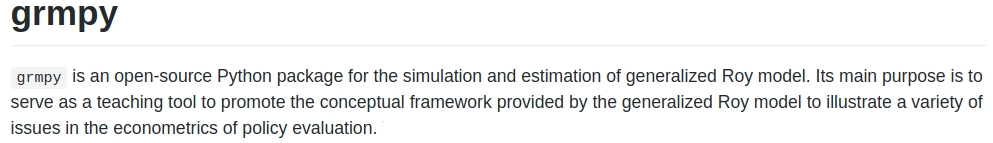
\includegraphics[scale=0.3]{../04_grmpy_tutorial_notebook/grmpy_intro.jpg}
\end{figure}
\end{frame}

\begin{frame}
\frametitle{\textit{grmpy}}

\begin{itemize}\setlength\itemsep{1em}
  \item \textit{\textbf{grmpy}} is ...
    \begin{itemize}\setlength\itemsep{1em}
      \item ...an open-source Python Package for the simulation and estimation of the generalized Roy model.
      \item ...intended as a useful device to support and improve the understanding of the framework by providing the opportunity to experience the effect of particular specifications directly.
    \end{itemize}
\end{itemize}
\end{frame}
